\documentclass[a4paper,12pt]{article}
\usepackage{graphicx}
\usepackage{caption}
\usepackage{subcaption}
\usepackage{float}
\usepackage[margin=1in]{geometry}
\usepackage{lmodern}
\usepackage{amsmath}
\usepackage{xcolor}
\usepackage{listings}
\usepackage{pgffor}

\lstset{
  breaklines=true,
  postbreak=\mbox{\textcolor{red}{$\hookrightarrow$}\space},
}

\graphicspath{{images/}}

\begin{document}

\title{Relatório kNN}
\author{Eduardo}
\date{\today}
\maketitle

A figura \ref{fig:dec_bound} mostra que a fronteira de decisão para um problema simples de gaussianas com pouca sobreposição é aproximadamente linear quando a quantidade de vizinhos considerada é adequada.

\begin{figure}[H]
  \centering
  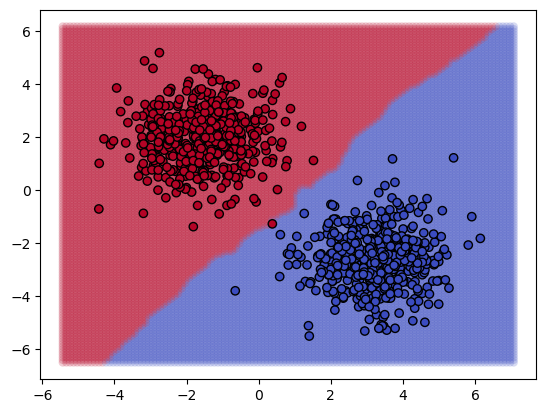
\includegraphics[width=0.8\textwidth]{decision_boundary.png}
  \caption{Fronteira de decisão para o classificador kNN com $k=5$}
  \label{fig:dec_bound}
\end{figure}

A matrix de precisão \ref{fig:acc_matrix} mostra que classificadores que consideram poucos vizinhos são suficientes para conjuntos de dados com pouca sobreposição. Entretanto, quanto maior o ruído, mais vizinhos são necessários para mitigar a influência de outliers.

\begin{figure}[H]
  \centering
  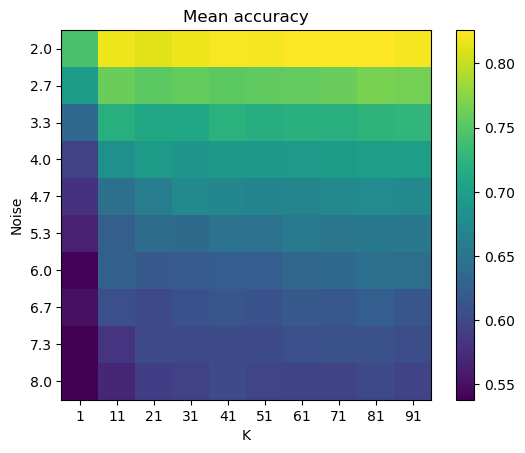
\includegraphics[width=0.8\textwidth]{k_noise_acc.png}
  \caption{Matriz de precisão para o classificador kNN}
  \label{fig:acc_matrix}
\end{figure}

\end{document}